\chapter{Experimentos}

\section{Análise Exploratória}

\subsection{Distribuição das classes}

Antes de mais nada, analisaremos a composição do nosso conjunto de dados e como se dá
a distribuição de classes. Na figura \ref{fig:classes} temos um histograma das classes associadas
a cada tuíte.

\begin{table}[H]
	\begin{center}
		\begin{tabular}{| l | l |}
			\hline
			Classe & Total \\
			\hline
			Positivo & 115 \\
			\hline 
			Negativo & 1248 \\ 
			\hline
			Neutro & 1223 \\ 
			\hline
		\end{tabular}
	\end{center}
	\caption*{Quantidade de tuítes pertencentes a cada classe}
	\label{tab:distribution}
\end{table}

\begin{center}
	\begin{figure}[H]
		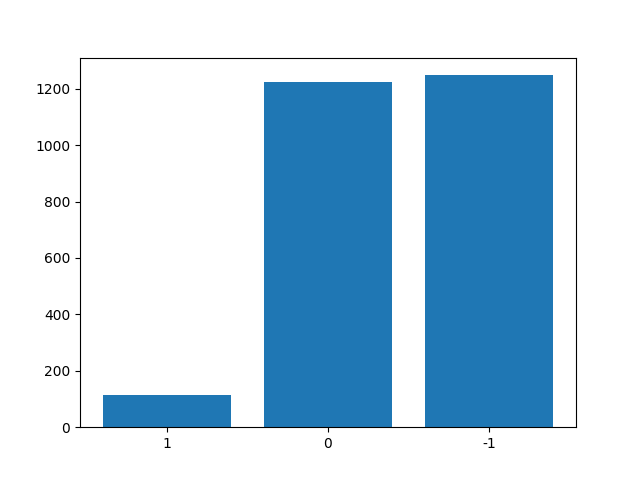
\includegraphics[scale=0.8]{fig_classes}
		\caption{Histograma da frequência de tuítes}
		\label{fig:classes}
	\end{figure}
\end{center}

Como podemos observar a partir da figura \ref{fig:classes} e tabela \ref{tab:distribution}, temos
que enquanto as classes negativa e neutra possuem distribuição próxima (48,26\% e 47,29\% 
respectivamente) a classe positiva corresponde a apenas 4,45\% de todos os tuítes. Mais a frente
veremos que esse desbalanceamento entre as classes irá acarretar em um desempenho ruim por parte
dos algoritmos de classificação, sejam os desenvolvidos para este trabalho quanto os da biblioteca
\texttt{scipy}.

\subsection{Características dos tuítes de cada classe}

A fim de entender como os classificadores realizariam o treinamento, analisou-se o conjunto de
dados a procura de padrões de características para cada classe.

Para os tuítes avaliados como neutro, notou-se o padrão que são tuítes derivados de portais de 
notícias ou são indagações, porém sem nenhuma crítica feita nelas.
A tabela abaixo mostra como exemplo alguns tuítes avaliados como neutro.

\begin{center}
	\begin{tabular}{| l | p{0.8\linewidth} |}
		\hline
		usuário & tuíte \\
		\hline
		Tica_Fernandes & Cidades têm protestos contra reforma da Previdência e terceirização http://g1.globo.com/politica/noticia/cidades-tem-protestos-contra-reforma-da-previdencia-e-terceirizacao.ghtml \\
		\hline
		andrcolett & Transposição do rio São Francisco, reforma do ensino médio/ da previdência , operação carne fraca, terceirização ... Enem vai bombar esse ano \\
		\hline
		VictoorAugustoo & Via @estadao : Manifestantes protestam em capitais do País contra reforma da Previdência e terceirização - http:/ln.is/estadao.com.brb29w1 \\
		\hline
		EdmilsonPequeno & O meu deputado @luizcoutopt votou contra a terceirização e é contra a reforma da previdência \\
		\hline
	\end{tabular}
\end{center}

Já para os tuítes negativos, nota-se a presença de palavrões e xingamentos 
junto de algumas \textit{hashtags} de cunho negativo como por exemplo \#ForaTemer,
além disso é comum a presença de tuítes onde as pessoas são convocadas para manifestações.
Outros termos comuns são escravidão e retrocesso, referindo-se diretamente às reformas da previdência e terceirização.

\begin{center}
	\begin{tabular}{| l | p{0.8\linewidth} |}
		\hline
		usuário & tuíte \\
		\hline
		MgracaGalvao & Dória é o maior Fake de todos os tempos. Se f... Palhaço \\
		\hline
		adamastaquio & Acorda POVO trabalhador. Previdencia + Terceirização + Reforma da CLT é P*** NO RABO DO POVO! \#ReformaTrabalhistaNÃO \\
		\hline
		TheMairaBastos & Reforma da previdência , desmonte da CLT, terceirização ,congelamento de gastos com a saúde e educação \#ForaTemerLadrao \#TemerGolpista \\
		\hline
		neyeverest & O PT esteve no poder por 14 anos o bandido do Lula e a burra da Dilma e o país está um caos pela instituição a roubalheira deles também !! \\
		\hline
		carinasotero & GREVE GERAL DIA 28/04 CONTRA RETROCESSOS DE TEMER • Reforma da Previdência • Reforma Trabalhista • Terceirização irrestrita \\
		\hline
	\end{tabular}
\end{center}

Assim como para os tuítes classificados como negativo, os tuítes positivos também eram 
caracterizados pela presença de \textit{hashtags}. Sejam elas declarando apoio a um candidato
(como \#Aecio2018 ou \#Lula2018) ou simplesmente manifestando alguma opinião positiva. 

\begin{center}
	\begin{tabular}{| l | p{0.8\linewidth} |}
		\hline
		usuário & tuíte \\
		\hline
		Verinha_Lu & É Aécio pelo Brasil !!! \#AécioPresidenteDoBrasil2018 \#EstamosComAécio \#DeusÉmaior e \#VitóriaVem \#FÉ \#SouAécio \\
		\hline
		Haddad_Femando & O salário mínimo aumentou 71\% durante os governos Lula e Dilma \#BrasilQueOPovoQuer \\
		\hline
		rovisacro & A favor da terceirização e tmb da reforma da previdência ! Mas óbvio, de forma justa e igualitária para todos, principalmente na previdência \\
		\hline	
	\end{tabular}
\end{center}

\section{Descrição dos experimentos}

Realizou-se duas etapas de experimentos, uma primeira etapa utilizando todas as classes onde se
observou que a baixa quantidade de elementos da classe positiva acabava por atrapalhar o desempenho
geral dos algoritmos, em especial os que utilizavam a abordagem OVA para o caso de multiclasses.
Com isso, decidiu-se descartar esses elementos e rodar uma nova sequência de experimentos 
considerando apenas as classes negativa e neutra (que para efeito dos algoritmos será a classe 
positiva) e, com isso, verificar a melhoria dos algoritmos nas métricas.

Para ambas as etapas, procurou-se não só medir o desempenho dos algoritmos, mas também encontrar
uma escolha certa de parâmetros para os mesmos que obtivesse a melhor performance (como a escolha
do Kernel no caso do SVM ou a constante de regularização usada tanto no SVM quanto na regressão
logística).

Tais testes de escolha de parâmetro, caso feitos usando apenas a divisão do conjunto de dados entre
conjunto de treino e conjunto de testes acabaria por dar uma escolha enviesada de parâmetros, uma
vez que uma escolha de parâmetros que tenha bons números em determinado conjunto de testes não
indica que ele possui uma boa generalização, isto é, apresentará uma boa precisão para novos dados.

A fim de garantir maior generalização, utiliza-se um método de validação chamado de 
validação cruzada, que se consiste de um modo de dividir o conjunto de dados e testá-lo com
um conjunto de validação. Uma primeira abordagem da validação cruzada seria dividir nosso conjunto
em três: um de treino, um de validação e outro de teste, assim testaríamos as escolhas de parâmetros
no conjunto de treino e, por fim, mediríamos a performance do melhor no conjunto de teste.

Outra abordagem seria ainda manter a divisão do conjunto de dados em conjunto de treino e teste
porém realizar esse procedimento diversas vezes alternando as porções que irão corresponder a
cada conjunto. Tal método é chamado de k-fold. No k-fold divide-se o conjunto total em k partições
e, a cada iteração, é construído um conjunto de teste usando uma das partições enquanto as k-1
serão o de treino. O procedimento de treinamento é realizado k vezes e, a escolha de parâmetros
com melhor desempenho médio será a escolhida. A figura \ref{fig:kfold} mostra o funcionamento do
método.

\begin{figure}[H]
	\begin{center}
		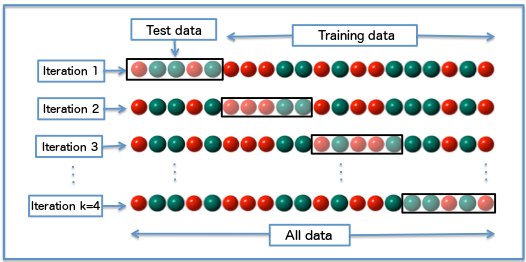
\includegraphics[scale=0.8]{K-fold_cross_validation}
	\end{center}		
	\caption{Funcionamento do método k-fold da validação cruzada \\
		fonte: \url{https://en.wikipedia.org/wiki/Cross-validation_(statistics)\#/media/File:K-fold_cross_validation_EN.jpg}}
	\label{fig:kfold}
\end{figure}



\section{Métricas avaliadas}

Para a realização dos experimentos, levou-se em consideração três métricas
para avaliar a eficiência dos classificadores.